\documentclass[a4paper,12pt,oneside]{article}

% \usepackage{graphicx}
% \usepackage{verbatim}
% \usepackage{amsmath}
% \usepackage[english]{babel}
% \usepackage[colorlinks,bookmarks=false,linkcolor=blue,urlcolor=blue]{hyperref}
% \usepackage{booktabs}

\usepackage{graphicx}
\usepackage{verbatim}
\usepackage{amsmath}
\usepackage[utf8]{inputenc}
\usepackage[colorlinks,bookmarks=false,linkcolor=blue,urlcolor=blue]{hyperref}
\usepackage{booktabs}
\usepackage{subfig}
\usepackage{amssymb}


\paperheight=297mm
\paperwidth=210mm

\setlength{\textheight}{235mm}
\setlength{\topmargin}{-1.2cm}
%\setlength{\footskip}{5mm}
\setlength{\textwidth}{15cm}
\setlength{\oddsidemargin}{0.56cm}
\setlength{\evensidemargin}{0.56cm}

\pagestyle{plain}


\def \be {\begin{equation}}
\def \ee {\end{equation}}
\def \dd  {{\rm d}}

\newcommand{\mail}[1]{{\href{mailto:#1}{#1}}}
\newcommand{\ftplink}[1]{{\href{ftp://#1}{#1}}}


\begin{document}

\title{Physique des couches minces}
\author{Laurent Rohrbasser \& Tim Tuuva}

\maketitle
\tableofcontents
\baselineskip=16pt
\parindent=15pt
\parskip=5pt


\newpage

% \begin{abstract}
% %Résumé de l'expérience, on fait des tps sur le chaos, rappeler vite fait 
% %dire le but de ces manips, qu'est ce qu'on veut?
% \end{abstract}

\section{Introduction}
Il est possible de faire des dépôts de très faibles épaisseur sur des surfaces quelconques relativement lisses. En plus de ne prendre qu'un espace relativement petit, les couches minces ont des propriétés utiles dans le domaine de l'électronique, et la protection aux interfaces d'un autre matériau. Il sera étudié ici les différents résultats de dépot de ZnO par pulvérisation cathodique magnétron sur une plaque de verre pour une variation de la température de dépôt, ainsi que l'effet d'un recuit à différentes températures pour chaque échantillons des couches déposées aux température précédentes.

\section{Un peu de theorie, dipositif expérimental}

Une couche mince, comme son nom l'indique, est une fine couche d'un matériau sur une surface appelée substratqui a généralement une épaisseur variant de $1\AA$ à $10$ micromètres.

Dans les expériences qui suivent, il a été effectué un certain nombre de dépôts de ZnO sur une plaque de verre par pulvérisation cathodique magnétron. Le principe se décrit comme suit (cf fig \ref{fig:illustration_depot}): une cible de ZnO est installée dans une enceinte à vide, le subtrat, ici une plaque de verre, est installée en face, la cible étant exposée à la face sur laquel il est souhaité faire le dépot. Ensuite un gaz réagissant peu (un gaz noble par exemple, ici de l'argon) est introduit dans l'enceinte et une grande différence de potentiel est imposée entre la cible et le substrat. Ceci a pour effet d'arracher un électron de l'argon et donc de le séparer en $Ag^+ + e^-$ et donc d'accélérer les particules $Ag^+$ contre la cible, en transférant de l'energie à la cible, des particules $Zn^+$ et $O^-$ quittent la cible pour se diriger vers la plaque de verre et se recristalliser. Un champ magnétique redirige les particules arrachées de la cible vers la zone où se trouve la plaque de verre. Chaque particule qui arrive sur la surface du verre pourra se déposer en un point et commencer un cluster de particules, se déposer à côté d'une particule ou d'un groupe de particules et ainsi participer à l'agrandissement d'un cluster (cristallisation), diffuser sur la plaque ou réévaporer, ainsi que toutes les combinisons possibles (cf fig \ref{fig:illustration_depot2}).

\begin{figure}[h!]
	\begin{center}
	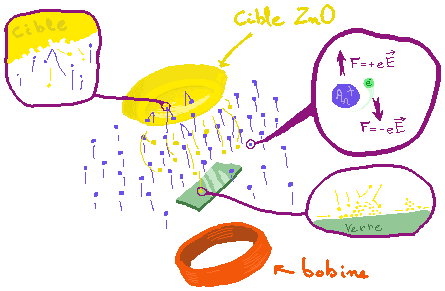
\includegraphics[width=1.\linewidth,angle=0]{./figures/illustration_depot.png}
	\caption{pulvérisation cathodique magnétron} \label{fig:illustration_depot}
	\end{center}
\end{figure}

\begin{figure}[h!]
	\begin{center}
	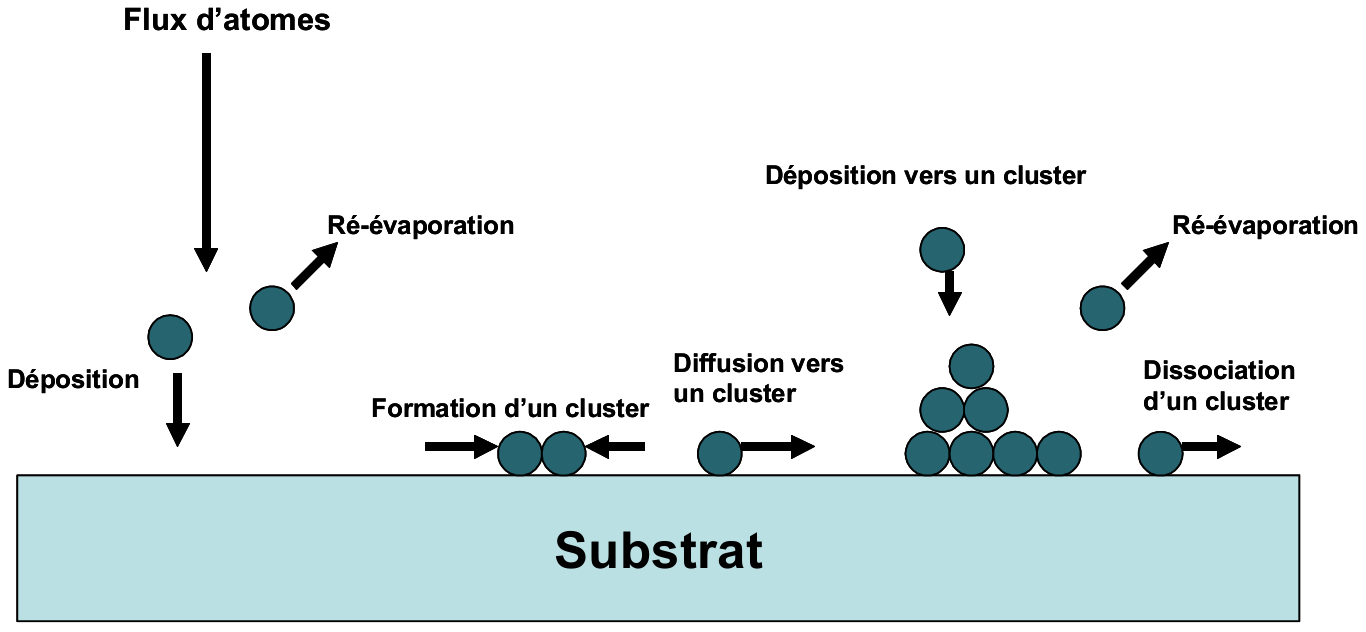
\includegraphics[width=1.\linewidth,angle=0]{./figures/illustration_depot2.png}
	\caption{différentes interractions pour une particule de la cible envoyée sur le substrat, à la surface du substrat} \label{fig:illustration_depot2}
	\end{center}
\end{figure}

Il est assez intuitif qu'il ne va pas se former un seul cristal sans défauts : les clusters peuvent commencer n'importe où avec des orientations différentes, et même au sein des clusters, on aura des défauts de substitution (un atome du cristal est remplacé par un autre atome), interstitielles (un atome se trouve inséré dans une position où on n'atend aucun atome) et lacunes (absence d'atome dans une position où on en attend un). Ces défauts ont des effets différents qui sont exploités pour faire ce qu'on appelle des dopages dans le cas de semi-conducteurs : en forcant l'introduction de particules étrangère on peut augmenter la densité d'électrons (dopage type N) ou la diminuer (dopage type P). Dans le cadre des expériences qui suivent, il sera étudié le ZnO qui est un semi-conducteur.


Dans le cadre des dépôts réalisés ici, on peut aussi considérer le ratio Zn - O : leurs affinités électronique étant différentes, ce ration aura un effet quand à la résistivité de l'échantillon. L'oxygène ayant une affinité électronique plus grande que le zinc, plus il y a de places occupées par des atomes d'oxygène dans le dépôt, plus le nombre d'électrons non mobiles sera grand et entrainera une rélusion des électrons mobiles, ce qui a pour effet de diffuser les électrons libres et donc d'augmenter la résistivité du milieu. Remplacer l'oxygène par du zinc permet donc de réduire la résistivité, et vice et versa.

Pour ajouter des particules dans le dépôt ou juste changer le rapport en nombre d'atomes Zn-O, il suffit d'ajouter dans l'enceinte l'élément souhaité avec le gaz noble. Par ailleurs, l'oxygene étant plus volatile que le zinc, pendant un dépôt on se retrouve facilement en déficite d'oxygene, on peut utiliser la procédure précédente pour réablir la stoechiométrie.


Comme dit précédemment, les cristaux ont non seulement des défauts ponctuels, mais aussi ne sont pas un unique cristal. En effet, vu que pendant le dépôt il se forme un grand nombre de clusters de ZnO, il se forme de nombreux petits cristaux, tous orientés différemment. Pour agir sur la façon dont se fait cette cristallisation, on peut faire un dépôt à une température différente : avec l'agitation thermique, une particule qui se dépose sur la plaque de verre se verra transmettre de l'énergie cinétique (depuis le verre) et aura plus de chance d'être redirigée vers un cluster déjà existant et donc ne va pas créer un autre début de cristal : la taille moyenne des cristaux va augmenter. Avec ceci on s'attend à ce qu'il soit plus facile pour les électrons de passer d'un point à l'autre de la couche mince (plus de régularité diminue le nombre de collisions), on peut mesurer la résistivité en fonction de la température du dépôt pour vérifier cela, de plus on peut faire une diffraction par rayon X pour comparer la taille des cristaux qu'on trouve dans le dépôt.

Il y a encore une autre solution pour agir sur la taille des cristaux : on peut a posteriori recristalliser la couche mince en faisant un recuit. Lors d'un recuit, les particules reçoivent de l'énergie et deviennet mobiles, ainsi les dislocations deviennent mobiles et les particules aux joins de grains (contact entre les différents petits cristaux) peuvent changer d'alignement. Il peut être observé que les cristaux les plus gros ont tendance à s'agrandir alors que les petits diminuent de taille avant de disparaître. 



% - expliquer la reformation des microcristaus en un gros cristal a haute temperature
% --- pourquoi les gros cristaux grandissent et les petits raptississent ?

% - pourquoi depot a chaud change
% --- energie de la plaque de verre transmise dans les particules de Zn, ainsi les Zn regagnent de l'energie et peuvent se mettre dans des endroits ou leur potentiel est plus faible.

% differents depots : Temperature
% 	- change l'energie fournue a la particule envoyee sur le substrat (favorise la formation de gros cristaux)
% recuit
% 	- change la taille des cristaux (recristalisation)


Une application possible des couches minces semi-conducteur est la diode photovoltaique : dans un dépôt mince de semi-conducteur sur un autre semi-conducteur (en faisant un contact N-P) ou sur un métal (diode Schottky) le fait que la couche soit mince permet à la lumière de le traverser, et ainsi, par le principe inverse d'une diode luminescente, de produire une différence de potentiel à partir d'un flux de photons. 


\subsection{resistivite (methode Van der Pauw)}
	La méthode devan der Pauw fonctionne sur des échantillons plats, homogène et de faible épaisseur. On prends 4 points de contacts comme dans la figure \ref{fig:illustration_van_der_pauw}, et on applique sur toutes les combinaisons possibles un courant et on mesure la tension entre les autres contacts restant (à un signe près) ce qui permet de calculer la résistivité avec la relation
	\be
		\rho = \frac{\pi}{ln 2} d R_{moyen}  F(R_1/R_2)
	\ee
	où d est l'épaisseur de l'échantillon, $R_{moyen}$ la moyenne des $R_1=V_{34}/I_{12}$ , $R_2=V_{41}/I_{23}$ , $R_3=V_{12}/I_{34}$ et $R_4=V_{23}/I_{41}$ et F est un facteur de correction pour un cas asymétrique, qui vaut 1 si le montage est réalisé comme dans la figure.
		\begin{figure}[h!]
			\begin{center}
			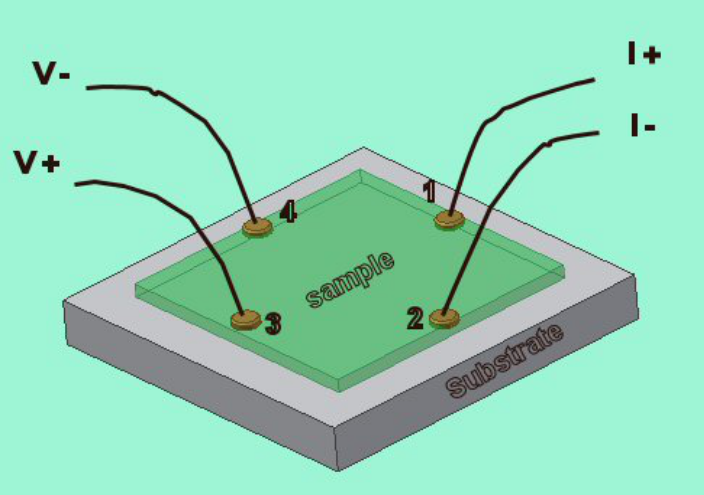
\includegraphics[width=.5\linewidth,angle=0]{./figures/illustration_van_der_pauw.png}
			\caption{Les contacts sont sur les sommets d'un carré pour avoir des distances identiques entre 1-3 et 2-4 ainsi que 1-2 et 2-3 et 3-4 et 4-1} \label{fig:illustration_van_der_pauw}
			\end{center}
		\end{figure}

\subsection{profilometre}
	Le profilomètre sert à mesurer l'épaisseur des couches minces sur les échantillons. Le processus consiste à faire un balayage de mesures de hauteur sur un chemin passant de la partie de la surface de l'échantillon qui a un dépôt jusqu'une partie qui a été converte pendant le dépôt (où il n'y a pas de couche mince). En mesurant les variations de l'épaisseur entre ces deux surfaces, on obtient l'épaisseur de la couche mince déposée.

\subsection{Effet Hall}
	L'effet Hall est la création d'une différence de potentiel lorsqu'on fait passer un courant dans un échantillon plongé dans un champ magnétique. La force de Lorentz appliquée aux électrons qui circulent dans l'échantillon implique une déviation des charges sur le côté et donc une différence de potentiel dans la direction orthogonale au courant (il faut que le champ ne soit pas aligné avec le courant).

	De la relation
	\be
		U_H = \frac{IB}{qNd}
	\ee
	où I est le courant imposé, B la valeur du champ lorsque celui ci est orthogonal à B, q la charge déplacée, d l'épaisseur de l'échantillon et N la densité de porteur de charges.

	Il est ainsi possible de calculer $N$ ainsi que la mobilité $\mu$ des porteurs de charge grâce à la relation
	\be
		\sigma = q N \mu
	\ee
	avec $\sigma=\rho^{-1}$ qui a pu être obtenu avec la méthode van der Pauw.

\subsection{spectre de reflexion}
% coeff absorption
% gap optique
!!!!!!!!!!!!!!!!!!!!!!!!!!!!!!!!!!!!!!!!!!!!!!!!!!!!!!!!!!
L'expérience consiste en envoyer de la lumière d'un spectre assez large, et de voir ce qui est réfléchi.

\be
	\omega_{min}=\sqrt{ \frac{q^2 N_{opt}} {\epsilon_0(\epsilon_\infty-1)m^*} }
\ee

ou $m^*$ est la masse effective de l'électron ($0.35 m_e$ pour le ZnO),





Avec le spectre de réflexion, il est aussi possible de mesurer l'épaisseur de l'échantillon : pour les longueur d'ondes les plus faibles, on constate un pattern régulier avec des interférences. Ces interférences sont due à la réflexion sur toute l'épaisseur de la lumière introduite. Pour la mesure de d, il suffit alors de regarder la distance entre 2 maximas donnés par $\lambda_1$ et $\lambda_2$, on utilise alors la relation :

\be
	d=\frac{M\lambda_1 \lambda_2}{2 n_f (\lambda_2 - \lambda_1)}
\ee


où $n_f$ est !!!!!!!!!!!!!!!!!!!!!!!!!!!!!!!!!!!!!!!!!!!!!!!!!!!

% \subsection{spectre de transmission}



\subsection{Diffraction rayonX}

		\begin{figure}[h!]
			\begin{center}
			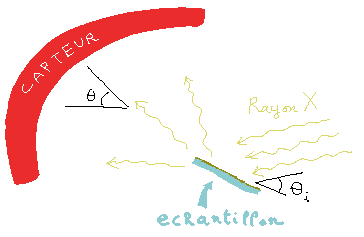
\includegraphics[width=0.8\linewidth,angle=0]{./figures/illustration_rayon_X.png}
			\caption{Les contacts sont sur les sommets d'un carré pour avoir des distances identiques entre 1-3 et 2-4 ainsi que 1-2 et 2-3 et 3-4 et 4-1} \label{fig:illustration_rayon_X}
			\end{center}
		\end{figure}

Dans cette partie, il est envoyé un faisceau de rayons X à un angle fixe sur l'échantillon, puis il est observé comment il est diffracté (cf figure \ref{fig:illustration_rayon_X}). Il est choisi un angle $\theta_i$ faible pour faire un sondage sur toute l'épaisseur de la couche mince. En mesurant l'intensité du faisceau selon l'angle $\theta$ comme montré dans la figure \ref{fig:illustration_rayon_X} , on constate l'existance d'angles avec des pics, ceci est dû à l'orientation des cristaux dans la couche : plus les pics sont nombreux et faibles, plus il y a d'orientation différentes.

Il se trouve qu'il y a une direction favorisée par la surface du verre sur lequel on fait le dépôt : il y a un pic permanent, plus ou moins large et plus ou moins haut. On peut utiliser pour ce picla relation de Deby-Scherrer pour estimer le volume moyen des cristaux dans le dépôt :

\be
	<z>_{vol}=\frac{K_s\lambda}{\beta^{hkl}_{1/2} cos\theta_{hkl}}
\ee

où $K_s$ est une constante dépendante de la géométrie de la cellule unitaire (typiquement comprise entre 0.85 et 0.99), $\lambda$ la longueur d'onde de la source de rayons X (il a été utilisé ici $Cu K_{\alpha}$ pour la source de rayons X, donc $\lambda = 1.5406 \AA$), $\beta^{hkl}_{1/2}$ la largeur à mi-hauteur du pic hkl de la diffraction et $\theta_{hkl}$ l'angle correspondant.



% \newpage
\section{résultats des expériences et discussion}

L'idée est de faire des dépôts à différentes températures pour observer vers quel état final tend la couche mince obtenue : il sera donc mesuré et comparé résistivité, épaisseur, taille des cristaux formés et densité de porteurs de charges libres par les méthodes décrites précédemment. Il sera aussi comparé les effets de recuits à différentes température.

Note : Dans l'ensemble des expérience, il a été ajouté dans l'enceinte du pulvérisateur cathodique magnétron un peu d'oxygène afin de rétablir la stoechiométrie pour le cristal ZnO : en effet, l'oxygène étant plus volatile que le zinc, on se retrouve avec un déficit en O. Malheureusement, le gaz introduit n'était pas purement de l'oxygène, mais une composition $21 \% O_2 $ et $78 \% N_2 $ et $1 \% $ de diverses impuretés.

Durant les dépôts à température supposément constante (donc chauffage éteint), il a pu être observé une augmentation de la température dans l'enceinte. Ceci peut s'expliquer par l'accélération des particules par le champ (cf fig \ref{fig:illustration_depot}) qui en percutant le support pour la plaque, lui transmet de l'energie et donc chauffe.

Dans la suite de ce document, les échantillons seront nommés selon leur température de dépôt et de recuit selon la règle suivante :

A correspond à un dépôt sans chauffage (température ambiante).

B correspond à un dépôt à $200^oC$.

C correspond à un dépôt à $400^oC$.

A1, B1 et C1 n'ont pas été recuit.

A2 a été recuit à $400^oC$.

A3, B2 et C2 ont été recuit à $600^oC$.
% +++ la temperature dans l'enceinte augmente avec le plasma

\subsection{Profilomètre}

\begin{table}[ht]
\centering
   \begin{tabular}{|c|c|}
	  \hline
      Type & Épaisseur [nm]\\
      \hline
      A & 571 \\
      B & 674 \\
      C & 872 \\
      \hline
   \end{tabular}
   \caption{autre tableau}\label{tab:profil}
\end{table}
On constate que l'épaisseur est du même ordre de grandeur. Les dépôts à haute température ont des épaisseurs différentes, ce qui est pricipalement dû à une différence dans les préparation : les temps de cuisson étants approximativement égaux, il est possible qu'une différence de l'ordre de la quintaine de minute ait pu contribuer à ces différences.

En plus de cela, le dépôt n'est pas complètement homogène : plus on est proche du centre, plus le dépôt est important, ce qui était visible à la couleur des couches minces obtenues pendant les expériences. Comme l'indique la figure \ref{fig:illustration_depot}, il y a bien un dispositif pour rediriger les particules de la cible (champ magnétique), mais il n'est pas parfait.

Pour les prochaines expérimentations, il peut être utile de mesurer les épaisseurs des dépôts en fonction de la position.

\subsection{Résistivité (methode Van der Pauw)}

s s s s s s s s s s s s s s s s s s s s s s s s s s s s s s s s s s s s s s s s s s s s s s s s s s s s s s s s s s s s s s s s s s s s s s s s s s s s s s s s s s s s s s s s s s s s s s s s s s s s s s s s s s s s s s s s s s s s s s s s s s s s s s s s s s s s s s s s s s s s s s s s s s s s s s s s s s s s s s s s s s s s s s s s s s s s s s s s s s s s s s s s s s s s s s s s s s s s s s s s s s s s s s s s s s s s s s s s s s s s s s s s s s s s s s s s s s s s s s s s s s s s s s s s s s s s s s s s s s s s s s s s s s s s s s s s s s s s s s s s s s s s s s s s s s s s s s s s s s s s s s s s s s s s s s s s s s s s s s s s s s s s s s s s s s s s s s s s s s s s s s s s s s s s s s s s s s s s s s s s s s s s s s s s s s s s s s s s s s s s s s s s s s s s s s s s s s s s s s s s s s s s s s s s s s s s s s s s s s s s s s s s s s s s s s s s s s s s s s s s s s s s s s s s s s s s s s s s s s s s s s s s s s s s s s s s s s s s s s s s s s s s s s s s s s s s s s s s s s s s s s s s s s s s s s s s s s s s s s s s s s s s s s s s s s s s s s s s s s s s s s s s s s s s s s s s s s s s s s s s s s s s s s s s s s s s s s s s s s s s s s s s s s s s s s s s s s s s s s s s s s s s s s s s s s s s s s s s s s s s s s s s s s s s s s s s s s s s s s s s s s s s s s s s s s s s s s s s s s s s s s s s s s s s s s s s s s s s s s s s s s s s s s s s s s s s s s s s s s s s s s s s s s s s s s s s s s s s s s s s s s s s s s s s s s s s s s s s s s s s s s s s s s s s s s s s s s s s s s s s s s s s s s s s s s s s s s s s s s s s s s s s s s s s s s s s s s s s s s s s s s s s s s s s s s s s s s s s s s s s s s s s s s s s s s s s s s s s s s s s s s s s s s s s s s s s s s s s s s s s s s s s s s s s s s s s s s s s s s s s s s s s s s s s s s s s s s s s s s s s s s s s s s s s s s s s s s s s s s s s s s s s s s s s s s s s s s s s s s s s s s s s s s s s s s s s s s s s s s s s s s s s s s s s s s s s s s s s s s s s s s s s s s s s s s s s s s s s s s s s s s s s s s s s 

\begin{table}[ht]
\centering
   \begin{tabular}{|c|c|c|c|c|c|c|c|c|}
	  \hline
      Type & I & $V_{3-4}$ & $V_{4-1}$ & $V_{1-2}$ & $V_{2-3}$ & Résistance& Résistivité\\
      &  [$\mu$A] & [mV] & [mV] & [mV] & [mV] & [$\Omega$] & [$\Omega$ m] \\
      \hline
      A1 & 30.003 & 0.41 & 1.92 & 0.421 & 2.24 & 0.176 & 100\ $10^{-9}$\\
      B1 & 30.004 & 0.349 & 0.426 & 0.370 & 0.431 & 0.06 & 40.44\ $10^{-9}$\\
      B2 & 30.004 & 2.463 & 1.170 & 2.409 & 1.180 & 0.27 & 182\ $10^{-9}$\\
      C1 & 29.996 & 0.62 & 2.29 & 0.62 & 2.30 & 0.22 & 192\ $10^{-9}$\\
      C2 & 30.004 & 3.08 & 1.22 & 3.18 & 1.37 & 0.33 & 288\ $10^{-9}$\\
      \hline
   \end{tabular}
   \caption{Tableau de la résistivité de la couche mince, par la méthode de Van Der Pauw}\label{tab:vanderpauw}
\end{table}



\subsection{Effet Hall}

L'expérience a causé un problème quand à la mesurabilité de l'effet : il n'a pas été possible de dinstinguer la différence de potentiel entre le moment où le champ magnétique était imposé et le moment où il n'y en avait pas, les variations étant plus faible que le bruit des appareils de mesure, il était impossible d'obtenir une variation de U. Le seul indice qu'il a pu être obtenu est que pour un champ de 1 Tesla, un courant de 32 mA (maximum qui a pu être imposé), les variations par rapport à un champ nul étaient en dessous de 0.001 mV. En plus de cela, les valeurs ne convergeant pas (l'échantillon chauffe) et il est pourtant nécessaire d'attendre après activation du champ magnétique car le bruit explose à ce moment.


\subsection{Spectre de réflexion}
s s s s s s s s s s s s s s s s s s s s s s s s s s s s s s s s s s s s s s s s s s s s s s s s s s s s s s s s s s s s s s s s s s s s s s s s s s s s s s s s s s s s s s s s s s s s s s s s s s s s s s s s s s s s s s s s s s s s s s s s s s s s s s s s s s s s s s s s s s s s s s s s s s s s s s s s s s s s s s s s s s s s s s s s s s s s s s s s s s s s s s s s s s s s s s s s s s s s s s s s s s s s s s s s s s s s s s s s s s s s s s s s s s s s s s s s s s s s s s s s s s s s s s s s s s s s s s s s s s s s s s s s s s s s s s s s s s s s s s s s s s s s s s s s s s s s s s s s s s s s s s s s s s s s s s s s s s s s s s s s s s s s s s s s s s s s s s s s s s s s s s s s s s s s s s s s s s s s s s s s s s s s s s s s s s s s s s s s s s s s s s s s s s s s s s s s s s s s s s s s s s s s s s s s s s s s s s s s s s s s s s s s s s s s s s s s s s s s s s s s s s s s s s s s s s s s s s s s s s s s s s s s s s s s s s s s s s s s s s s s s s s s s s s s s s s s s s s s s s s s s s s s s s s s s s s s s s s s s s s s s s s s s s s s s s s s s s s s s s s s s s s s s s s s s s s s s s s s s s s s s s s s s s s s s s s s s s s s s s s s s s s s s s s s s s s s s s s s s s s s s s s s s s s s s s s s s s s s s s s s s s s s s s s s s s s s s s s s s s s s s s s s s s s s s s s s s s s s s s s s s s s s s s s s s s s s s s s s s s s s s s s s s s s s s s s s s s s s s s s s s s s s s s s s s s s s s s s s s s s s s s s s s s s s s s s s s s s s s s s s s s s s s s s s s s s s s s s s s s s s s s s s s s s s s s s s s s s s s s s s s s s s s s s s s s s s s s s s s s s s s s s s s s s s s s s s s s s s s s s s s s s s s s s s s s s s s s s s s s s s s s s s s s s s s s s s s s s s s s s s s s s s s s s s s s s s s s s s s s s s s s s s s s s s s s s s s s s s s s s s s s s s s s s s s s s s s s s s s s s s s s s s s s s s s s s s s s s s s s s s s s s s s s s s s s s s s s s s s s s s s s s s s s s s s s s s s s s s s s s s s s s s s s s s s s s s s s s s s s s s s s s s s s s s 


\begin{figure}[!ht]
    \subfloat[A0 (dépôt à $20^\circ$C)\label{fig:refl_A0}]{
      \includegraphics[width=0.5\linewidth,angle=0]{./figures/A0.pdf}
    }
    % \hfill
    \subfloat[A1 (dépôt à $20^\circ$C)\label{fig:refl_A1}]{%
      \includegraphics[width=0.5\linewidth,angle=0]{./figures/A1.pdf}
      }\\
    \hfill
    \subfloat[A2 (dépôt à $20^\circ$C, recuit à $400^\circ$C)\label{fig:refl_A2}]{%
      \includegraphics[width=0.5\linewidth,angle=0]{./figures/A2.pdf}
      }
    \hfill
    \subfloat[B1 (dépôt à $200^\circ$C)\label{fig:refl_B1}]{%
      \includegraphics[width=0.5\linewidth,angle=0]{./figures/B1.pdf}
    }\\
	\begin{center}
    \subfloat[B2 (dépôt à $200^\circ$C, recuit à $600^\circ$C)\label{fig:refl_B2}]{
      \includegraphics[width=0.5\linewidth,angle=0]{./figures/B2.pdf}
    }
	\end{center}
    \subfloat[C1 (dépôt à $400^\circ$C)\label{fig:refl_C1}]{%
      \includegraphics[width=0.5\linewidth,angle=0]{./figures/C1.pdf}
      }
   % \hfill
    \subfloat[C2 (dépôt à $400^\circ$C, recuit $600^\circ$C)\label{fig:refl_C2}]{%
      \includegraphics[width=0.5\linewidth,angle=0]{./figures/C2.pdf}
    }
    \caption{Spectres de diffraction par rayonX des couches minces.}
    \label{fig:diff_main}
\end{figure}

\subsection{Diffraction rayonX}
s s s s s s s s s s s s s s s s s s s s s s s s s s s s s s s s s s s s s s s s s s s s s s s s s s s s s s s s s s s s s s s s s s s s s s s s s s s s s s s s s s s s s s s s s s s s s s s s s s s s s s s s s s s s s s s s s s s s s s s s s s s s s s s s s s s s s s s s s s s s s s s s s s s s s s s s s s s s s s s s s s s s s s s s s s s s s s s s s s s s s s s s s s s s s s s s s s s s s s s s s s s s s s s s s s s s s s s s s s s s s s s s s s s s s s s s s s s s s s s s s s s s s s s s s s s s s s s s s s s s s s s s s s s s s s s s s s s s s s s s s s s s s s s s s s s s s s s s s s s s s s s s s s s s s s s s s s s s s s s s s s s s s s s s s s s s s s s s s s s s s s s s s s s s s s s s s s s s s s s s s s s s s s s s s s s s s s s s s s s s s s s s s s s s s s s s s s s s s s s s s s s s s s s s s s s s s s s s s s s s s s s s s s s s s s s s s s s s s s s s s s s s s s s s s s s s s s s s s s s s s s s s s s s s s s s s s s s s s s s s s s s s s s s s s s s s s s s s s s s s s s s s s s s s s s s s s s s s s s s s s s s s s s s s s s s s s s s s s s s s s s s s s s s s s s s s s s s s s s s s s s s s s s s s s s s s s s s s s s s s s s s s s s s s s s s s s s s s s s s s s s s s s s s s s s s s s s s s s s s s s s s s s s s s s s s s s s s s s s s s s s s s s s s s s s s s s s s s s s s s s s s s s s s s s s s s s s s s s s s s s s s s s s s s s s s s s s s s s s s s s s s s s s s s s s s s s s s s s s s s s s s s s s s s s s s s s s s s s s s s s s s s s s s s s s s s s s s s s s s s s s s s s s s s s s s s s s s s s s s s s s s s s s s s s s s s s s s s s s s s s s s s s s s s s s s s s s s s s s s s s s s s s s s s s s s s s s s s s s s s s s s s s s s s s s s s s s s s s s s s s s s s s s s s s s s s s s s s s s s s s s s s s s s s s s s s s s s s s s s s s s s s s s s s s s s s s s s s s s s s s s s s s s s s s s s s s s s s s s s s s s s s s s s s s s s s s s s s s s s s s s s s s s s s s s s s s s s s s s s s s s s s s s s s s s s s s s s s s s s s s s s s s s s s 

\begin{figure}[!ht]
	\centering
    \subfloat[A2 (dépôt à $20^\circ$C, recuit à $400^\circ$C)\label{fig:diff_A2}]{
      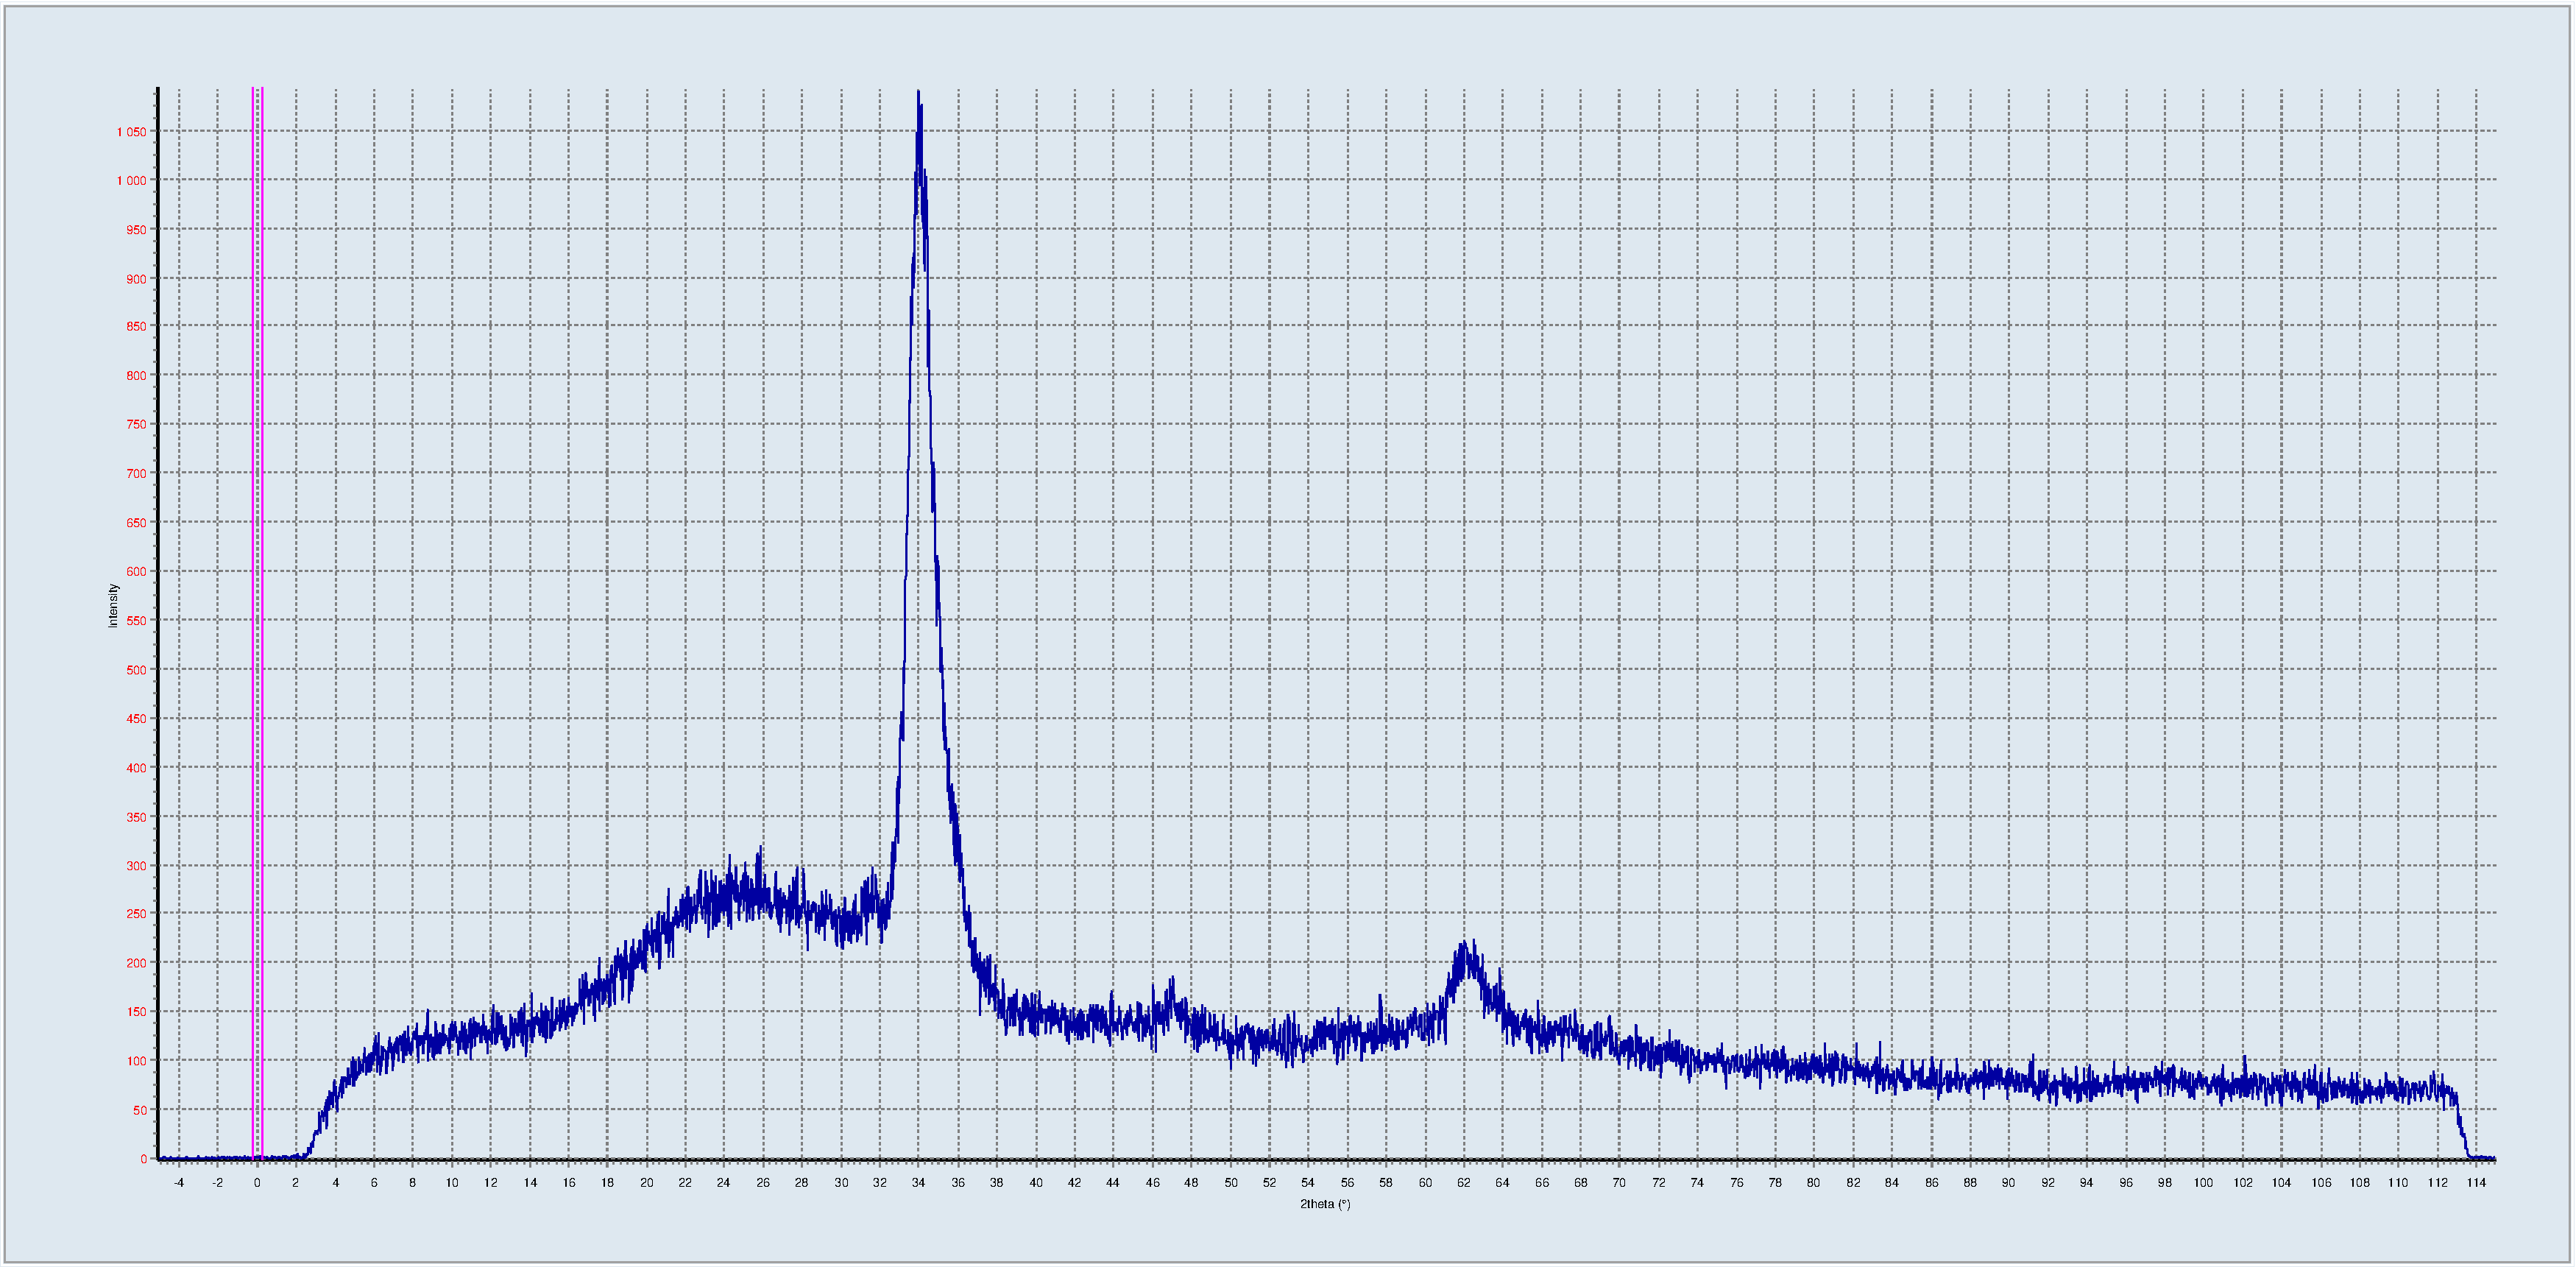
\includegraphics[width=0.5\linewidth,angle=0]{./data/graph/diffraction/A1_002.pdf}
    }\\
    \subfloat[A1 (dépôt à $20^\circ$C)\label{fig:diff_A1}]{
      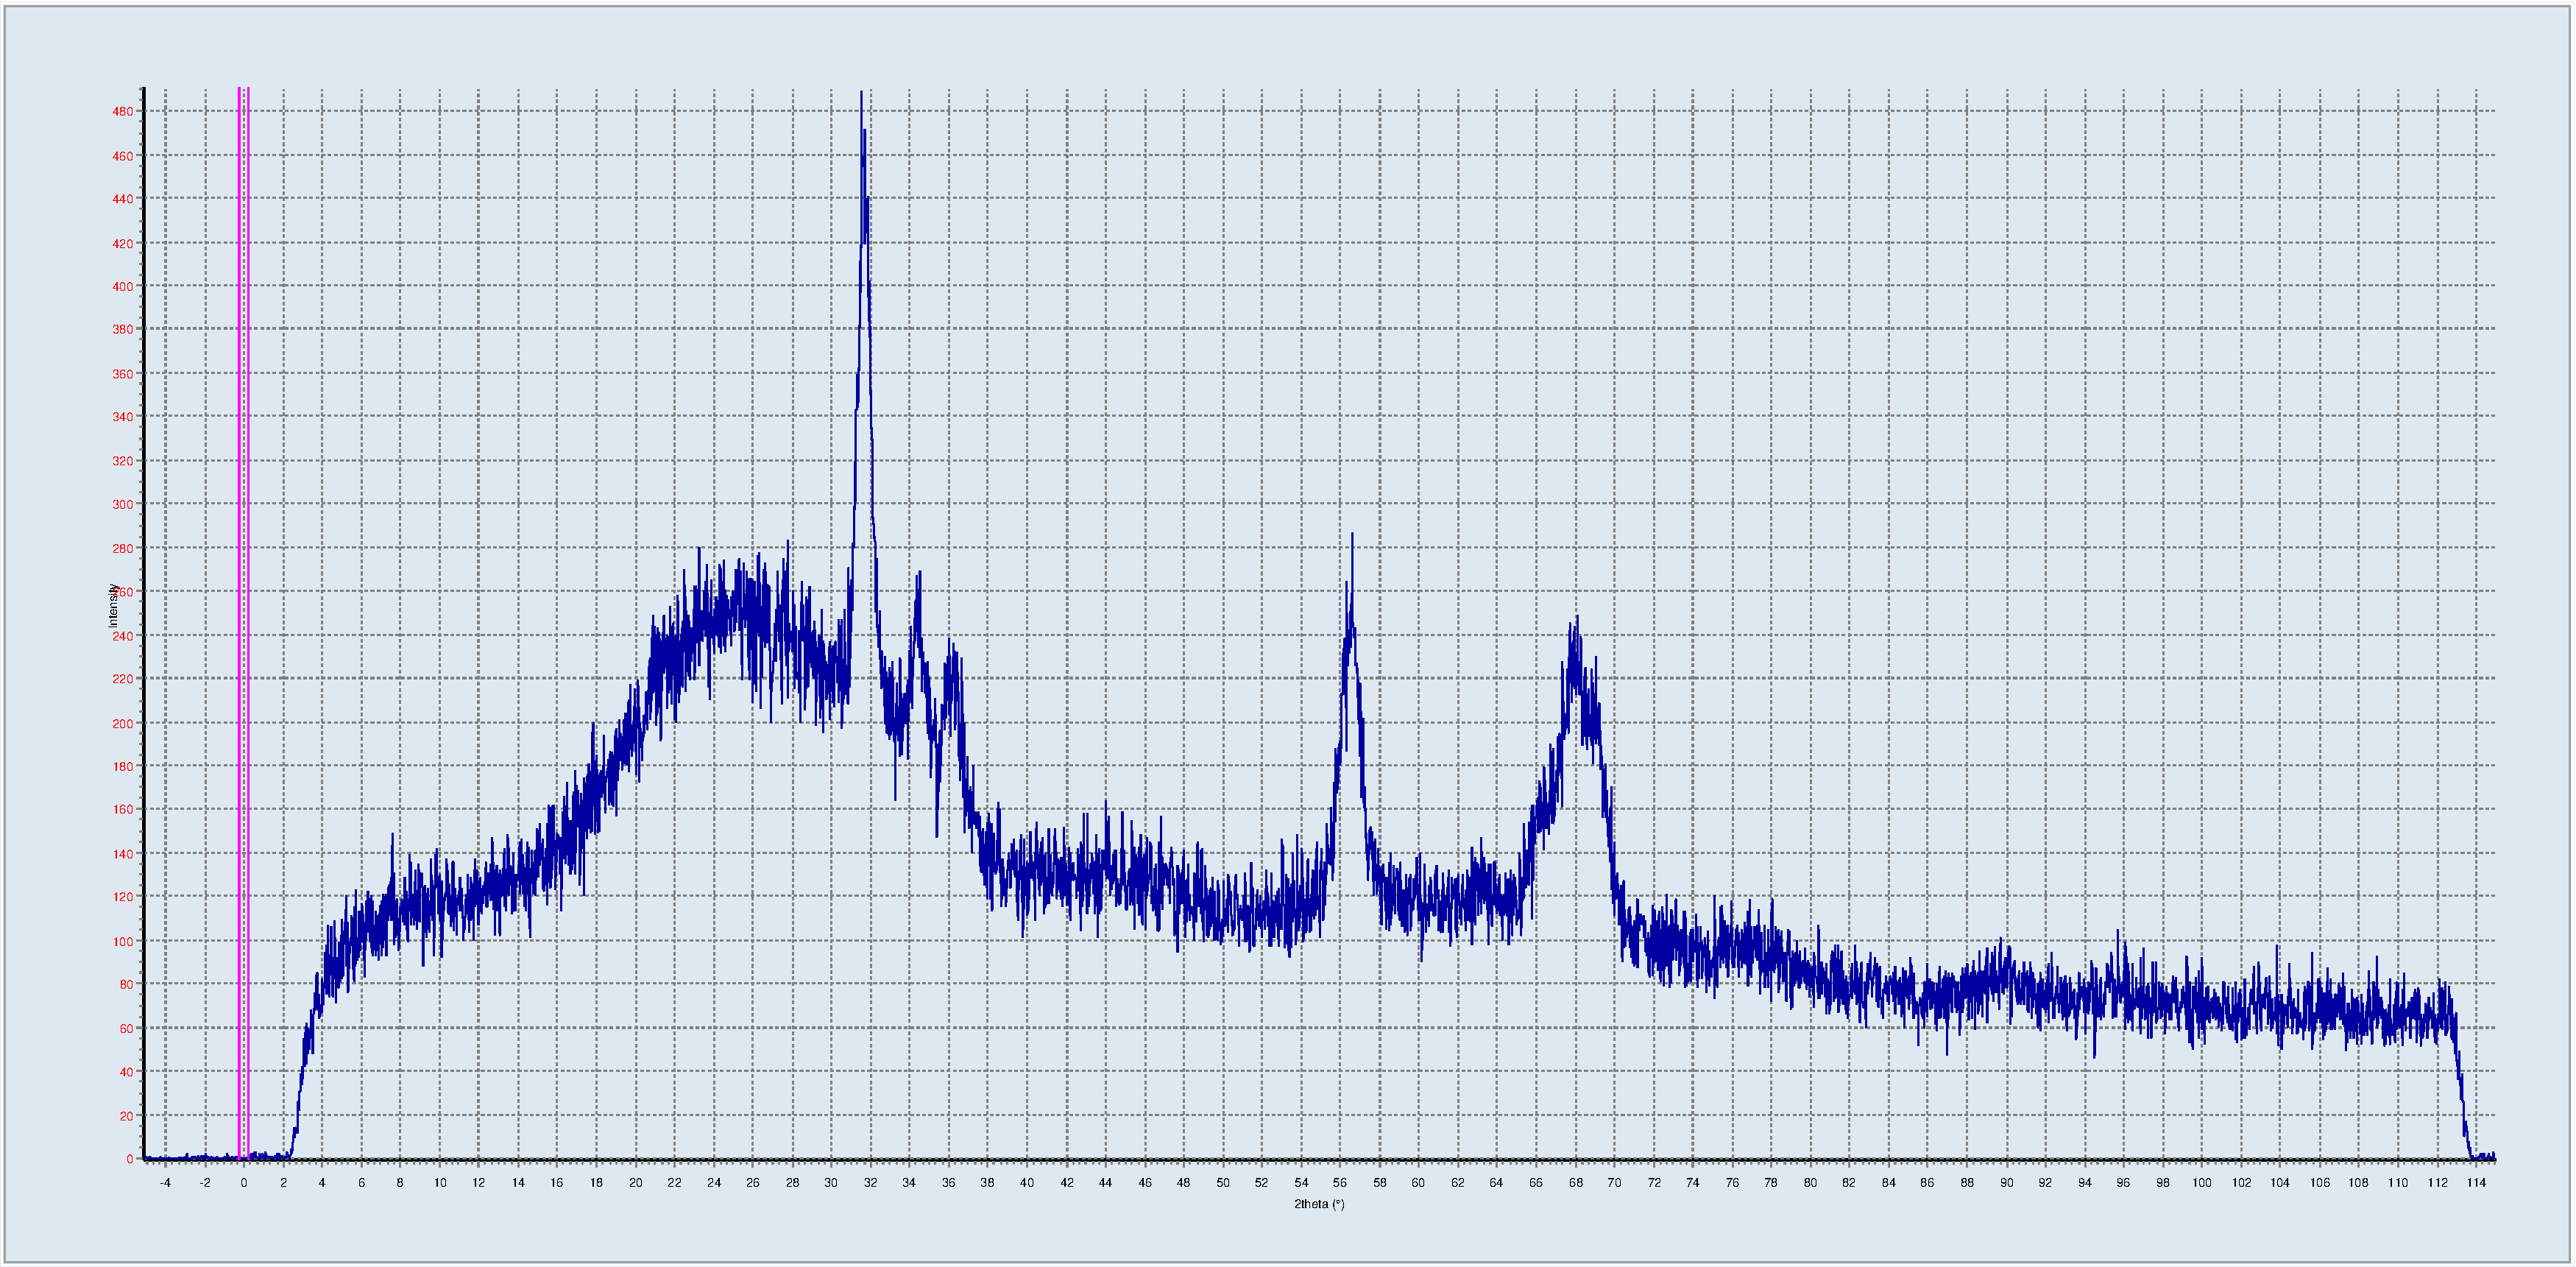
\includegraphics[width=0.5\linewidth,angle=0]{./data/graph/diffraction/A2_001.pdf}
    }
    % \hfill
    \subfloat[A3 (dépôt à $20^\circ$C, recuit à $600^\circ$C)\label{fig:diff_A3}]{%
      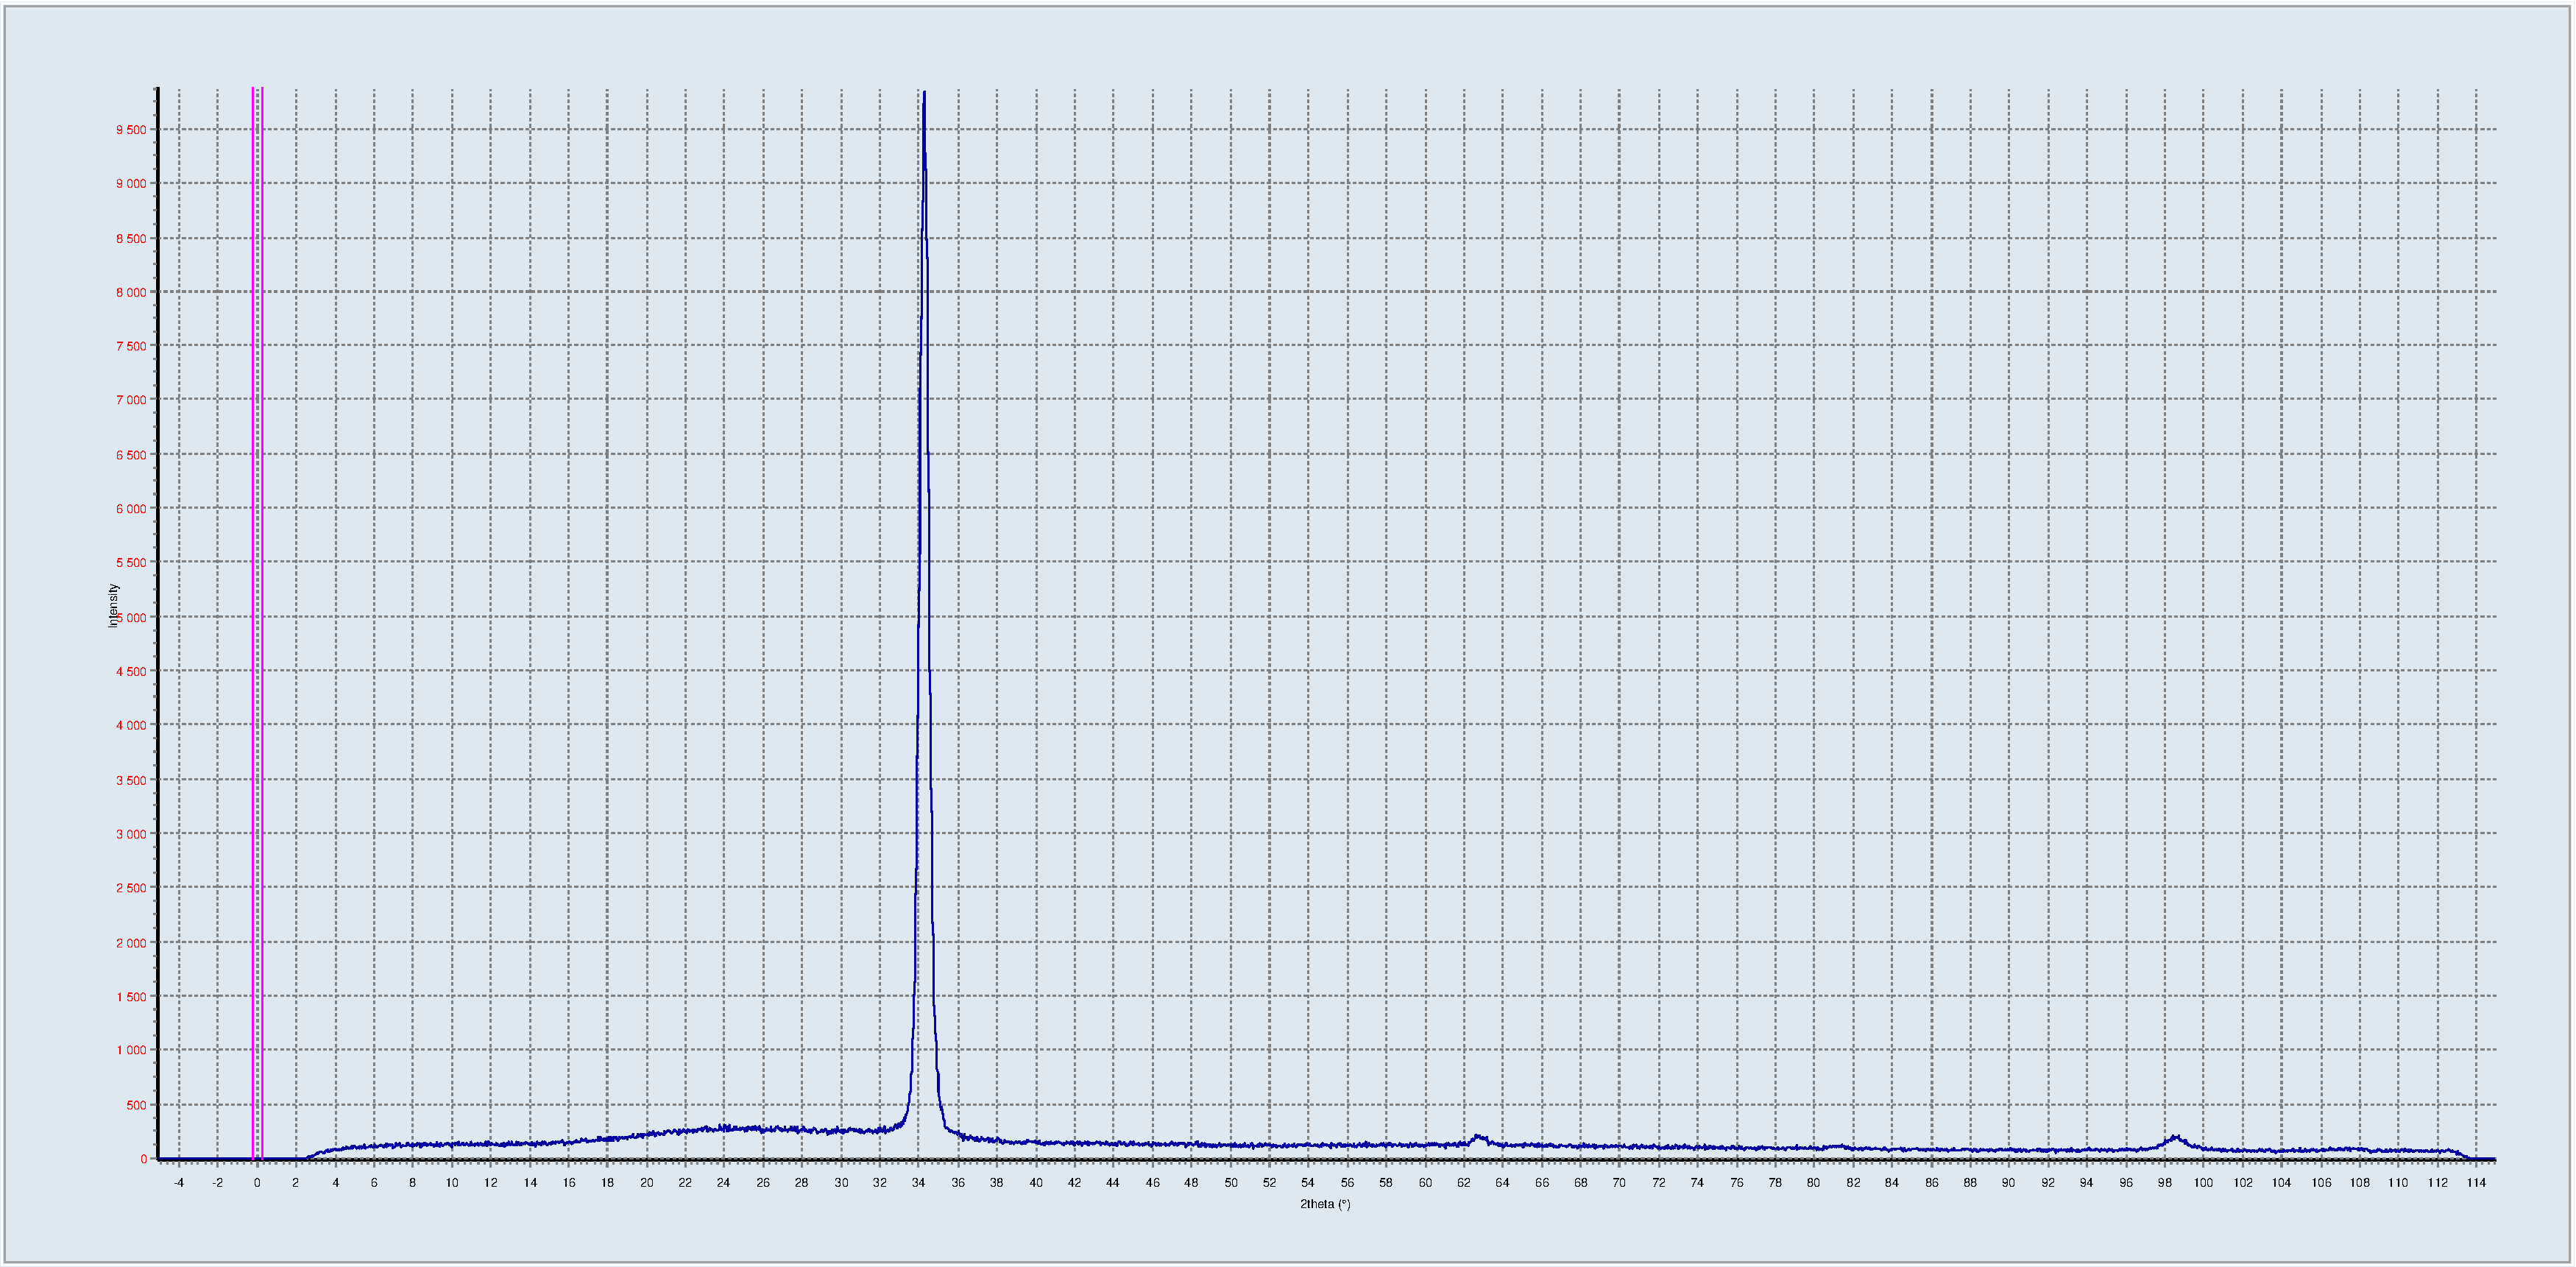
\includegraphics[width=0.5\linewidth,angle=0]{./data/graph/diffraction/A3_001.pdf}
      }\\
    \hfill
    \subfloat[B1 (dépôt à $200^\circ$C)\label{fig:diff_B1}]{%
      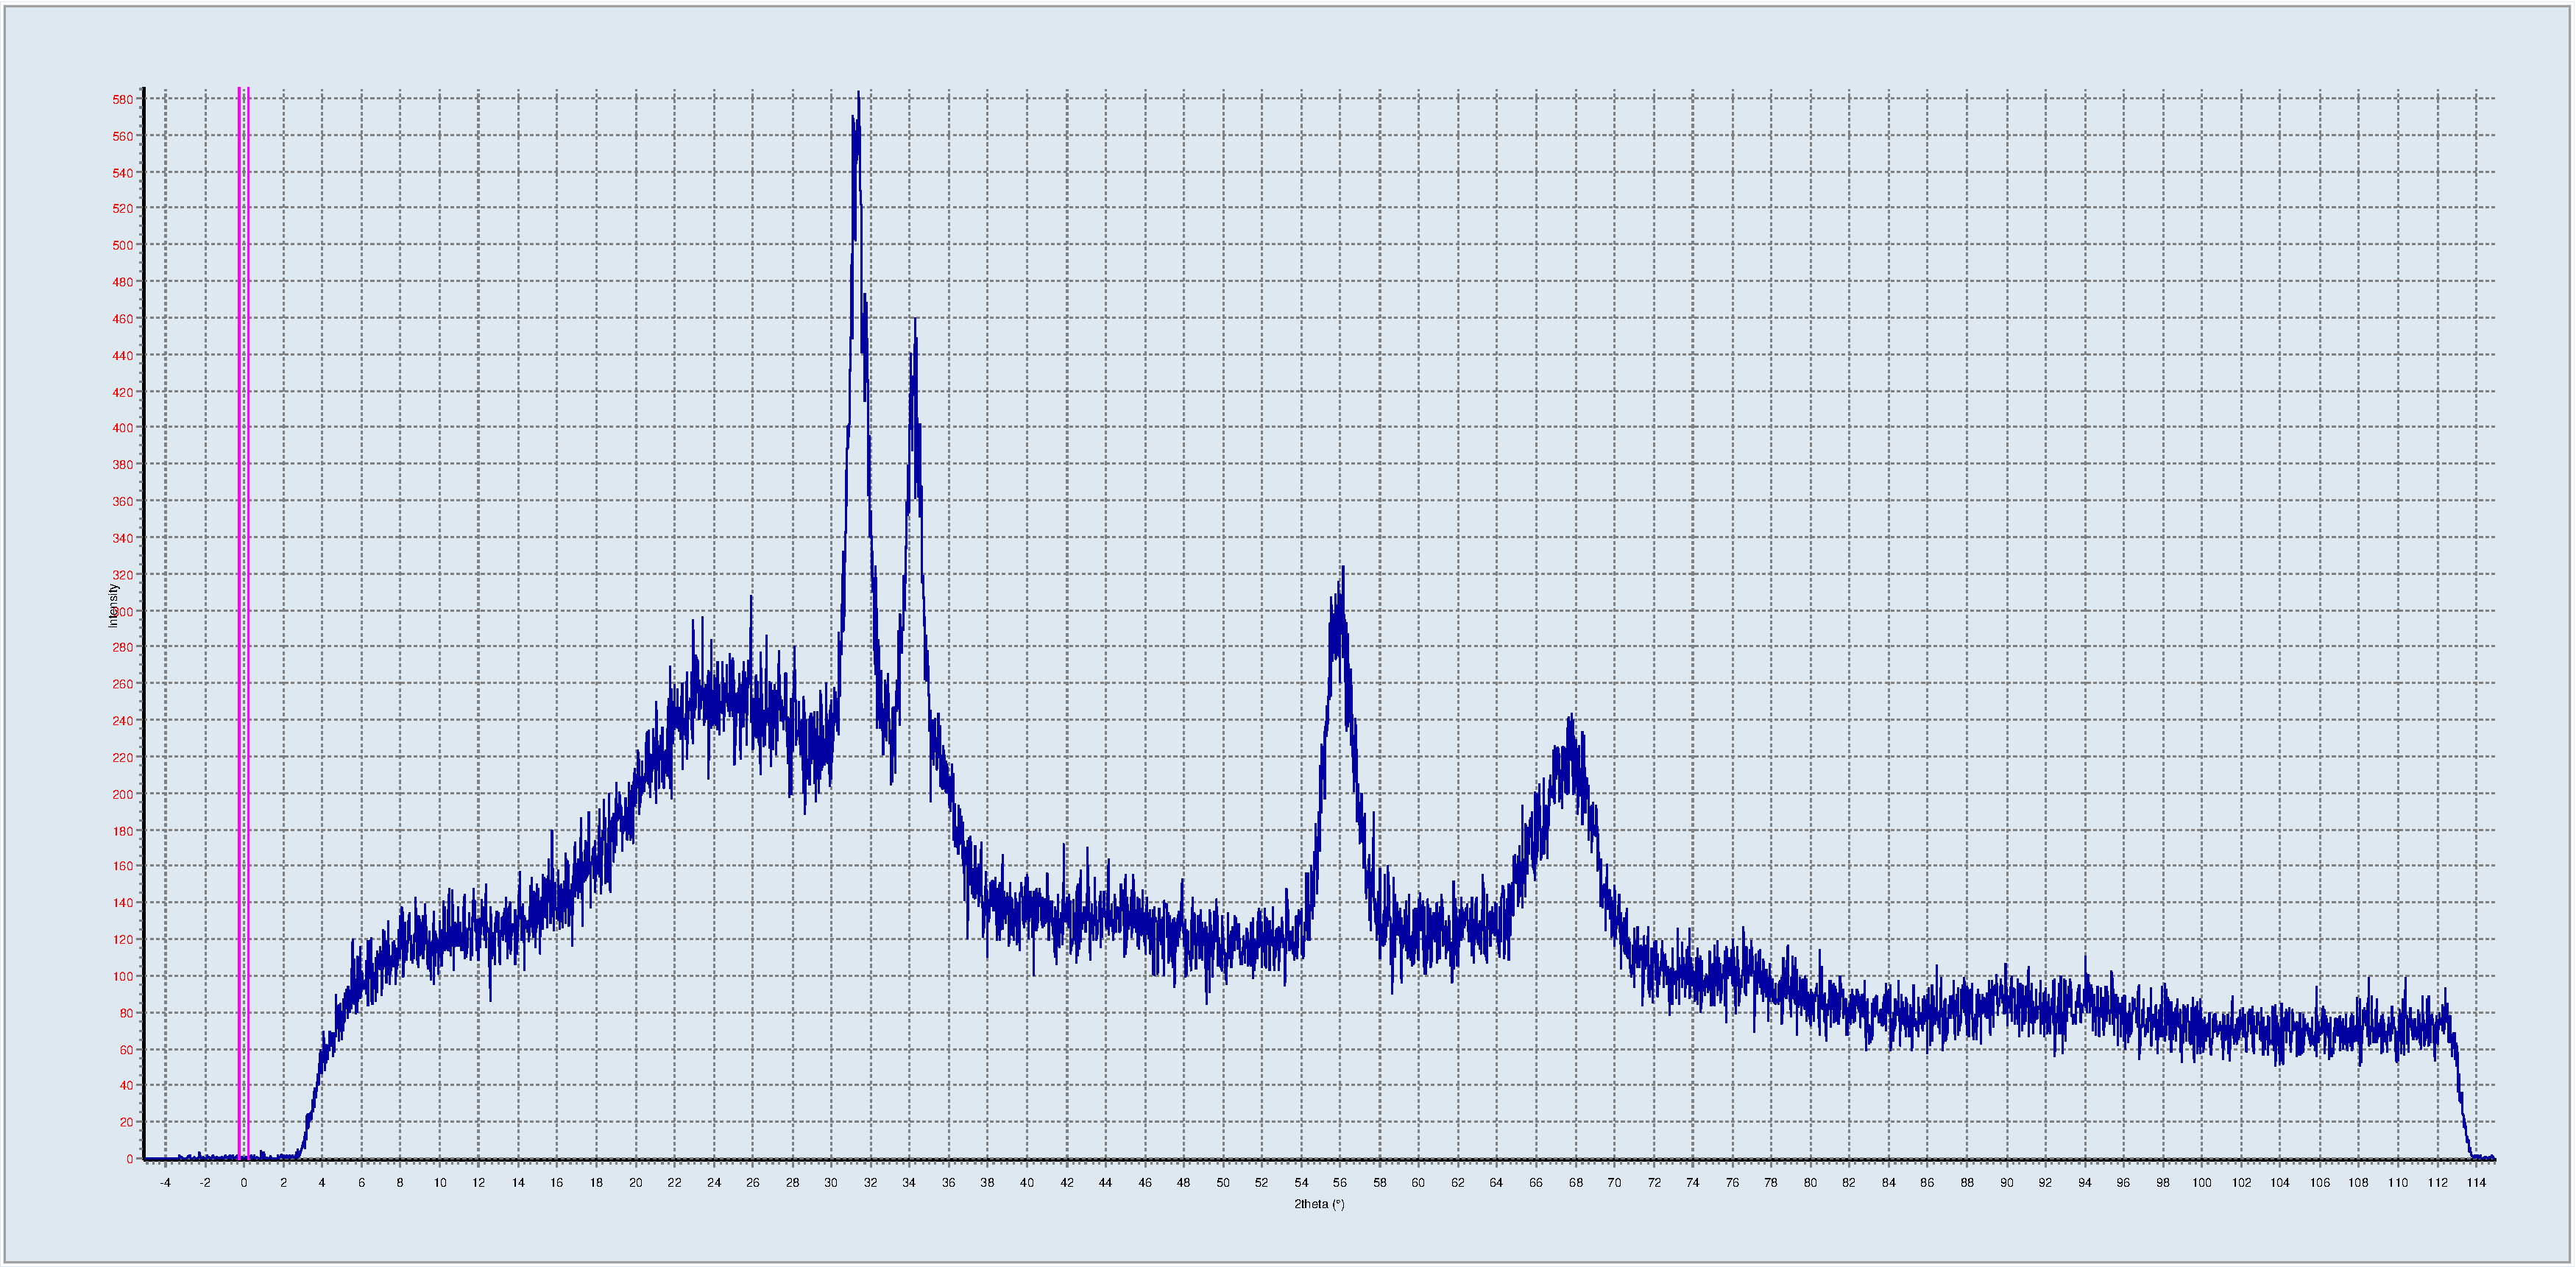
\includegraphics[width=0.5\linewidth,angle=0]{./data/graph/diffraction/B1_003.pdf}
    }
    \subfloat[B2 (dépôt à $200^\circ$C, recuit à $600^\circ$C)\label{fig:diff_B2}]{
      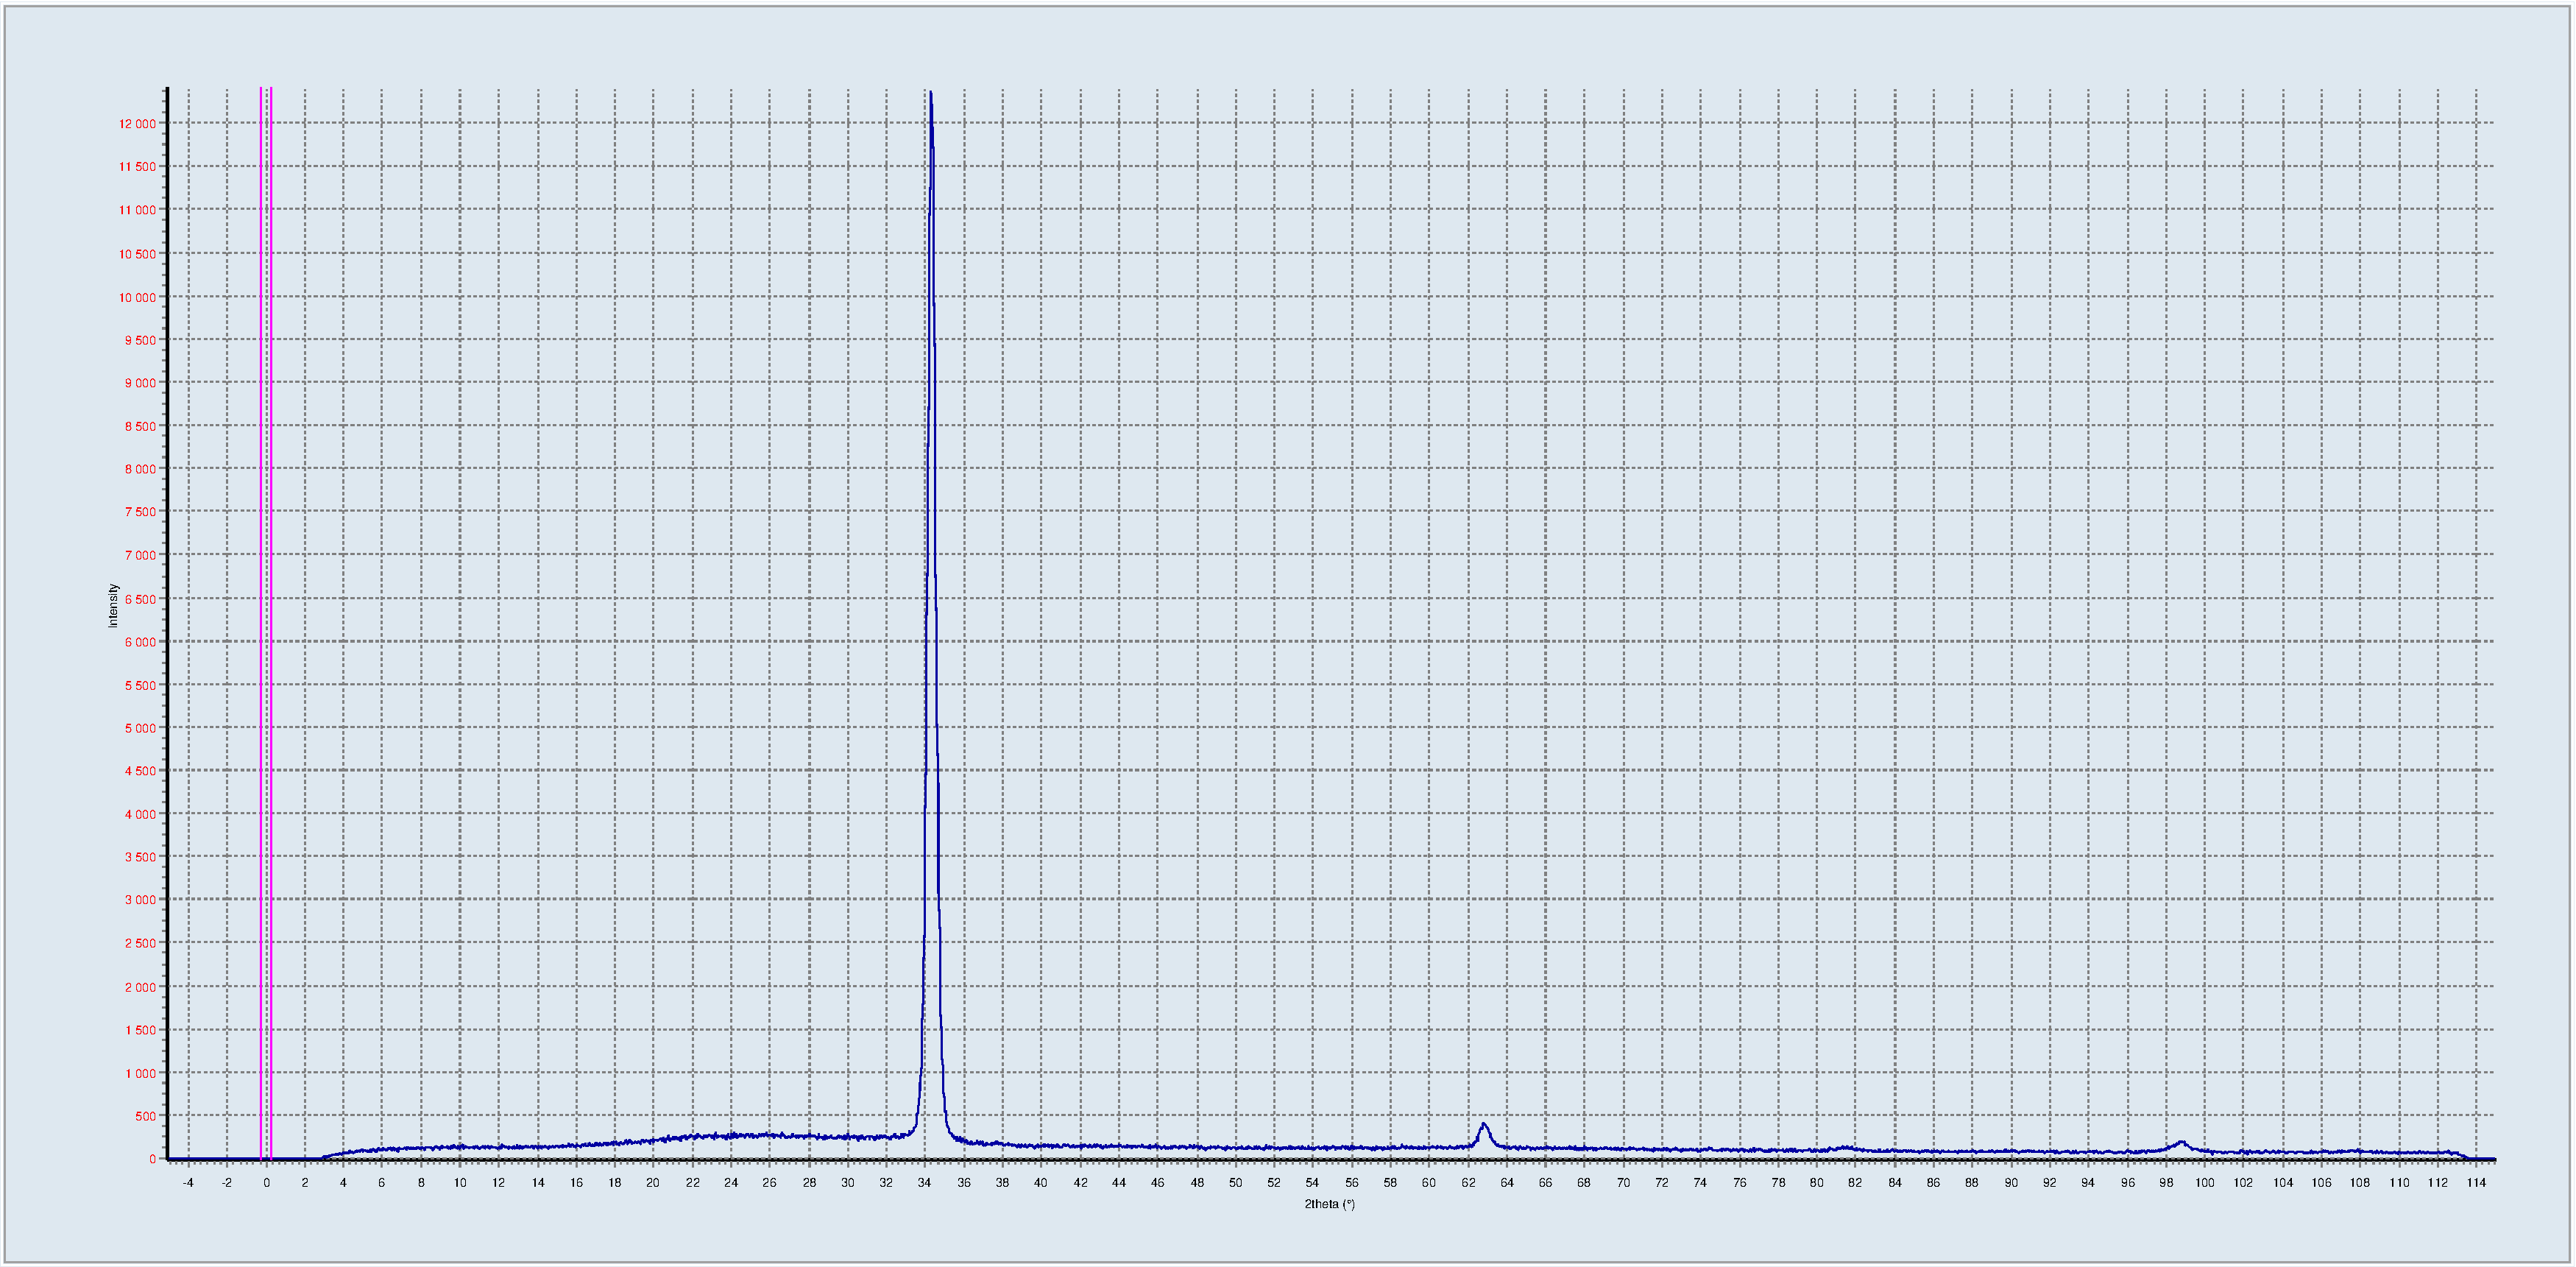
\includegraphics[width=0.5\linewidth,angle=0]{./data/graph/diffraction/B2_001.pdf}
    }\\
     \hfill
    \subfloat[C1 (dépôt à $400^\circ$C)\label{fig:diff_C1}]{%
      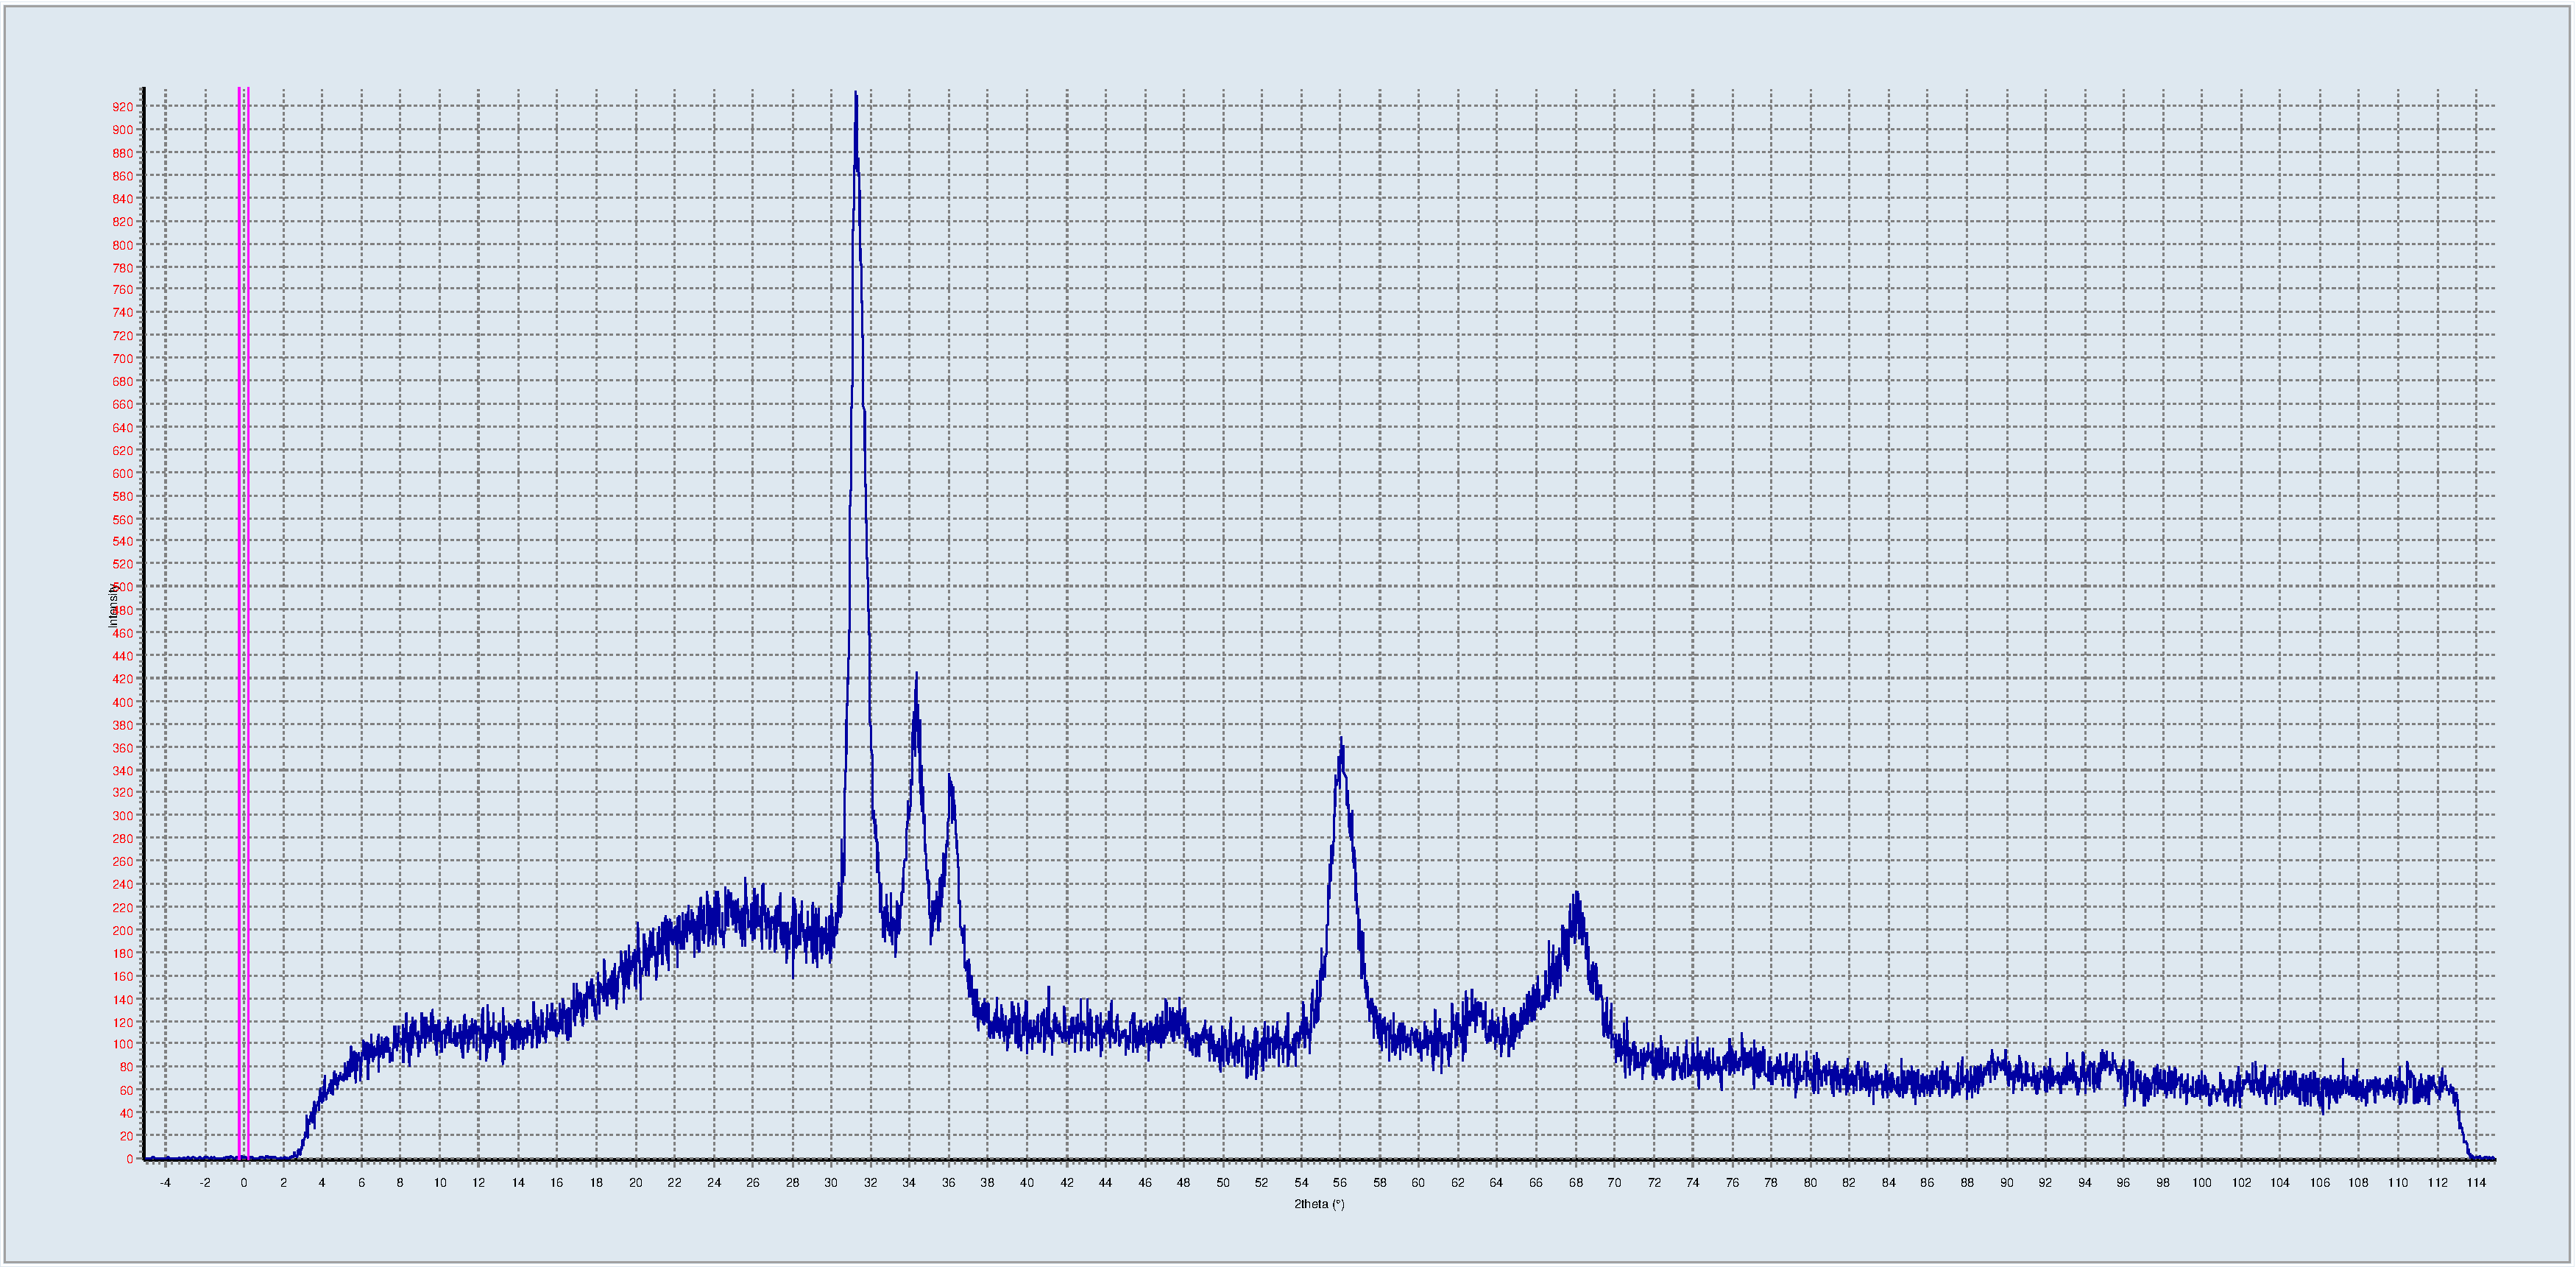
\includegraphics[width=0.5\linewidth,angle=0]{./data/graph/diffraction/C1_003.pdf}
      }
   % \hfill
    \subfloat[C2 (dépôt à $400^\circ$C, recuit $600^\circ$C)\label{fig:diff_C2}]{%
      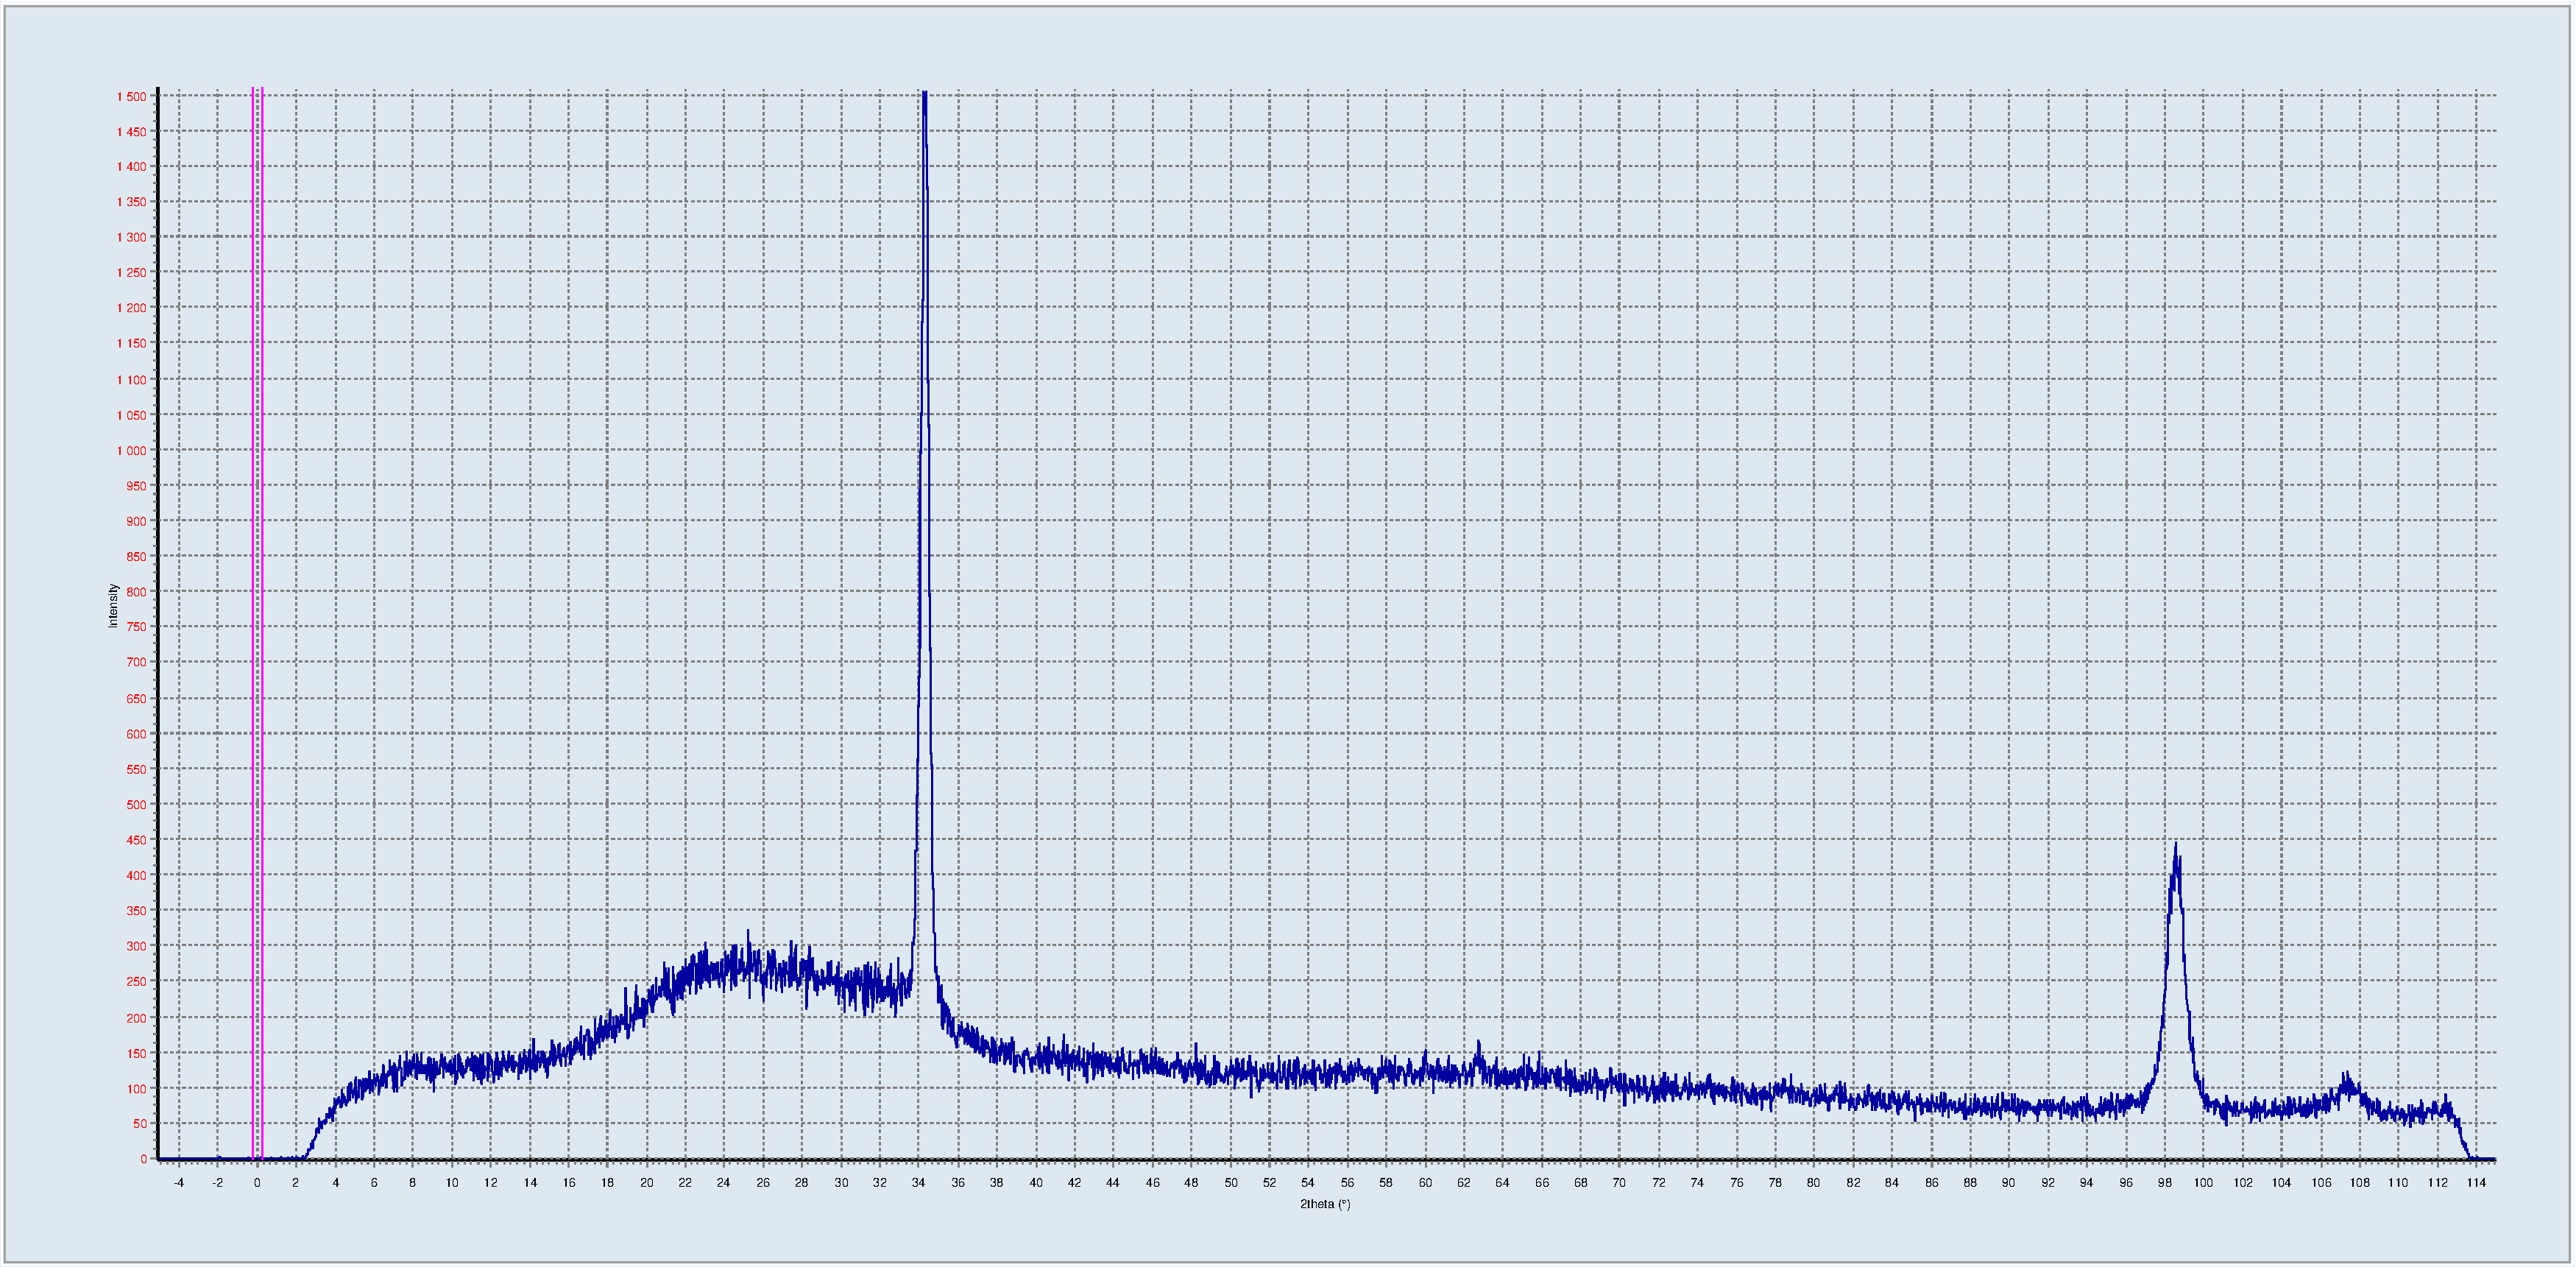
\includegraphics[width=0.5\linewidth,angle=0]{./data/graph/diffraction/C2_001.pdf}
    }
    \caption{Spectres de diffraction par rayonX des couches minces.}
    \label{fig:diff_main}
\end{figure}


\begin{table}[ht]
\centering
   \begin{tabular}{|c|c|}
	  \hline
      Type & $<z>$\\
      \hline
      A1 & 1.639 \\
      A2 & 1.594 \\
      A3 & 2.48 \\
      B1 & 2.409 \\
      B2 & 2.741 \\
      C1 & 2.437 \\
      C2 & 3.282 \\
      \hline
   \end{tabular}
   \caption{Tableau des mesures de $<z>$ via la diffraction par rayon X.}\label{tab:X}
\end{table}






% [x] A0 dépot 20° (No O2)
% [x] Ax dépot 20° (No O2) + recuit 400°

% [x] A1 dépot 20°
% [x] A2 dépot 20° + recuit 400°
% [x] A3 dépot 20° + recuit 600°

% [x] B1 dépot 200°
% [x] B2 dépot 200° + recuit 600°

% [x] C1 dépot 400°
% [x] C2 dépot 400° + recuit 600°



% résistivité
% [x]A0
% [ ]Ax
% [x]A1
% [ ]A2
% [ ]A3
% [ ]B1
% [ ]B2
% [x]C1
% [ ]C2

% épaisseur (profilomètre)
% [x]A0
% [!]Ax
% [x]A1
% [!]A2
% [!]A3
% [x]B1
% [!]B2
% [x]C1
% [!]C2

% concentration charge par effet Hall
% [?]A0
% [?]Ax
% [?]A1
% [?]A2
% [?]A3
% [?]B1
% [?]B2
% [?]C1
% [?]C2

% Spectre
% [x]A0
% [x]Ax
% [x]A1
% [ ]A2
% [x]A3
% [x]B1
% [x]B2
% [x]C1
% [x]C2

% Diffraction 
% [ ]A0
% [ ]Ax
% [ ]A1
% [ ]A2
% [ ]A3
% [ ]B1
% [ ]B2
% [ ]C1
% [ ]C2



\section{Conclusion}

%Résumer du rapport
%Ouverture





%Reference
\begin{thebibliography}{99}
\bibitem{la notice}
\end{thebibliography}

\end{document}
